\chapter{Podstawy teoretyczne}
\label{ch:podstawy-teoretyczne}


W niniejszym rozdziale przedstawiono kluczowe zagadnienia teoretyczne, które stanowią fundament techniczny realizowanego projektu. Przedstawienie podstaw działania zastosowanych elementów pozwoli lepiej zrozumieć wyzwania projektowe oraz przyjęte metody rozwiązywania problemów związanych ze sterowaniem i nawigacją mobilnej platformy robotycznej.

Omówione zostaną najważniejsze zasady funkcjonowania enkoderów kwadraturowych, które umożliwiają monitorowanie ruchu - podstawowej odometrii. Zaprezentowane zostaną także zasady działania regulatora PID, powszechnie stosowanego w układach sterowania.

W dalszej części omówiono wybrane algorytmy z zakresu wizji komputerowej, takie jak detekcja krawędzi i rozpoznawanie kolorów, które stanowią istotne elementy systemu wizyjnego robota.

\section{Enkodery}

Enkodery są urządzeniami pomiarowymi, które umożliwiają śledzenie ruchu obrotowego lub liniowego. W zastosowaniach z zakresu robotyki, takich jak opisywana platforma mobilna, enkodery umożliwiają śledzenie prędkości i pozycji, co jest kluczowe dla poprawnej implementacji odometrii – procesu śledzenia pozycji robota w przestrzeni. Enkodery dzielą się na enkodery optyczne, magnetyczne i mechaniczne, w zależności od zastosowanej technologii detekcji. W omawianym projekcie szczególne zastosowanie znajdują enkodery kwadraturowe, montowane przy silnikach odpowiedzialnych za napęd różnicowy robota.

\subsection{Rodzaje enkoderów}

Enkodery klasyfikowane są na podstawie zasady ich działania, co wpływa na precyzję pomiarów oraz możliwości aplikacyjne. Główne typy enkoderów to:

\begin{itemize}
    \item \textbf{Enkodery optyczne} - działają na zasadzie przerywania wiązki światła przez tarczę z otworami, generując impulsy odpowiadające ruchowi. Ten typ enkoderów charakteryzuje się dużą precyzją, co czyni je popularnym wyborem w robotyce.
    \item \textbf{Enkodery magnetyczne} - działają w oparciu o zmiany pola magnetycznego, zwykle generowane przez magnes przymocowany do osi. Zastosowanie efektu Hall'a w tych enkoderach pozwala na wykrywanie zmian w polu magnetycznym, co jest kluczowe w enkoderach kwadraturowych. Są wytrzymałe i odporne na kurz czy wibracje, przez co dobrze sprawdzają się w trudnych warunkach.
    \item \textbf{Enkodery mechaniczne} - najprostszy rodzaj enkoderów, wykorzystujący mechaniczne styki do generowania impulsów. Ze względu na ograniczoną trwałość są rzadziej stosowane w precyzyjnych aplikacjach.
\end{itemize}


\subsubsection{Efekt Hall'a}

Efekt Hall'a stanowi podstawę działania magnetycznych enkoderów kwadraturowych, a jego działanie opiera się na generowaniu napięcia (tzw. napięcia Hall'a) prostopadłego do kierunku przepływu prądu i linii pola magnetycznego. Gdy magnes jest umieszczony w pobliżu sensora Hall'a, zmiany pola magnetycznego wywołują impulsy wykrywane przez enkoder. W przypadku enkoderów kwadraturowych dwa czujniki Hall'a rozmieszczone pod kątem 90° umożliwiają rozróżnienie kierunku obrotu wału oraz precyzyjny pomiar przebytej odległości. Zastosowanie efektu Hall'a w enkoderach kwadraturowych daje możliwość tworzenia solidnych, odpornych na zużycie i precyzyjnych pomiarów.


\begin{figure}[h]
    \centering
    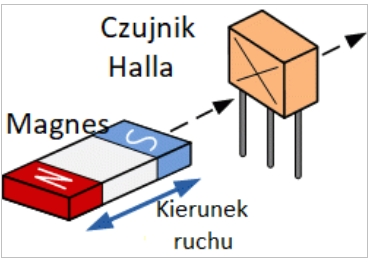
\includegraphics[width=0.5\textwidth]{./graf/halla-enc.jpg}
    \caption{Rysunek przedstawiający zasadę działania czujnika Hall'a \cite{bib:hall_net}}
    \label{rys2:encoders-graf}
\end{figure}

\subsection{Enkodery kwadraturowe}

Enkodery kwadraturowe to specjalny rodzaj enkoderów, które umożliwiają nie tylko pomiar prędkości i położenia, ale także kierunku obrotu. Składają się z dwóch sygnałów wyjściowych – A i B – przesuniętych względem siebie o fazę 90°. Dzięki temu fazowemu przesunięciu system sterujący jest w stanie określić kierunek obrotu, analizując, który z sygnałów A lub B wyprzedza drugi. Każdy impuls generowany przez sygnały A i B odpowiada określonemu przemieszczeniu kątowemu, co pozwala na wyznaczenie pozycji kątowej osi obrotu z wysoką precyzją.


\begin{figure}[h]
    \centering
    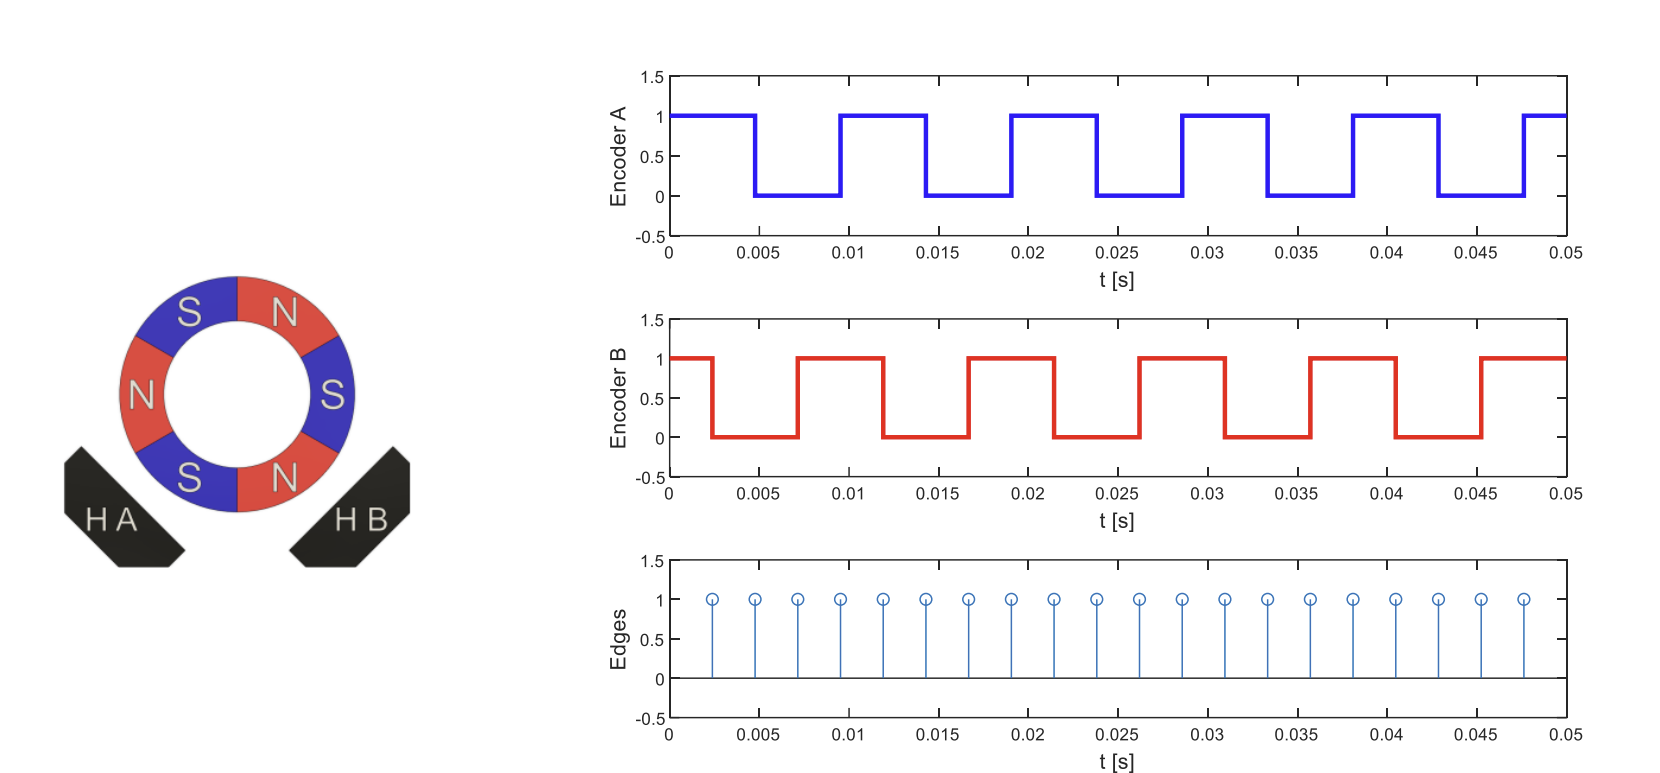
\includegraphics[width=0.8\textwidth]{./graf/enkoders.png}
    \caption{Rysunek przedstawiający ideowo budowę enkodera kwadraturowego oraz sygnałów przez niego generowanych \cite{bib:encoders-pid}}
    \label{rys2:encoders-graf}
\end{figure}


\begin{figure}[h]
    \centering
    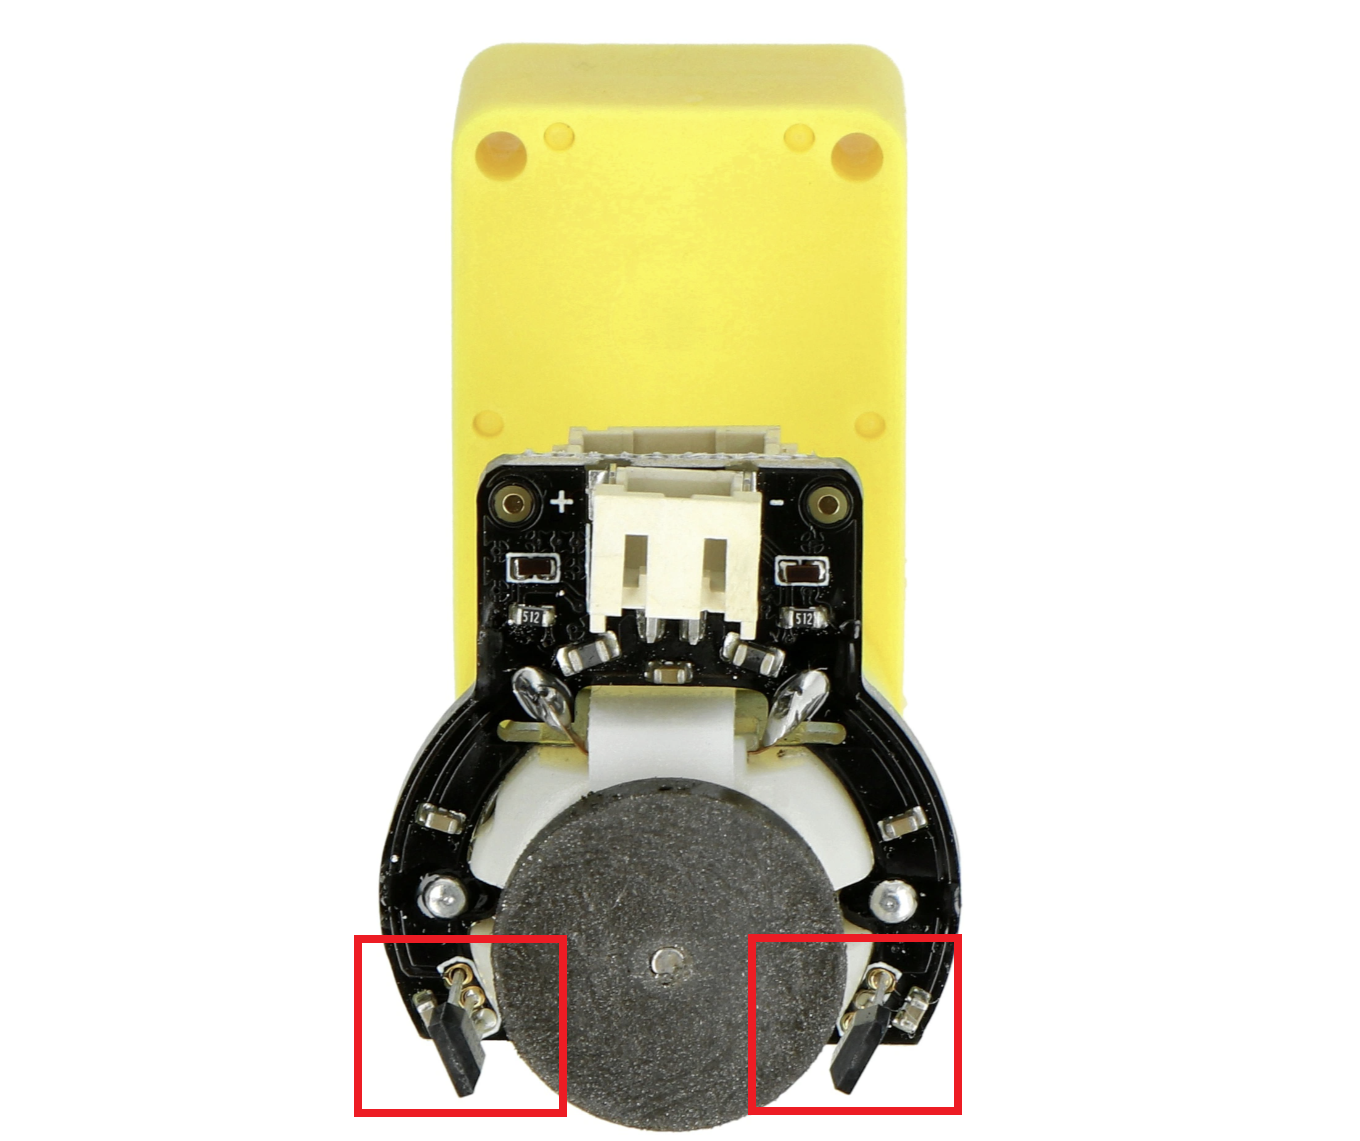
\includegraphics[width=0.5\textwidth]{./graf/enkoder-silnik.png}
    \caption{Rysunek przedstawiający przykładowy wygląd enkodera opartego o efekt Hall'a. Czerwonymi kwadratami są zaznaczone tranzystory wykrywające zmianę pola magnetycznego podczas obrotu wału \cite{bib:botland-hall}}
    \label{rys2:encoders-graf}
\end{figure}

\clearpage

\section{Regulator PID}

Regulator PID (ang. \textit{Proportional-Integral-Derivative}) jest jednym z najczęściej stosowanych regulatorów w systemach automatycznego sterowania, ze względu na swoją prostotę implementacji oraz skuteczność w wielu aplikacjach przemysłowych i robotycznych. Regulator ten wykorzystuje trzy składniki: proporcjonalny, całkujący oraz różniczkujący.

\subsection{Ogólny schemat układu regulacji}

\begin{figure}[h]
    \centering
    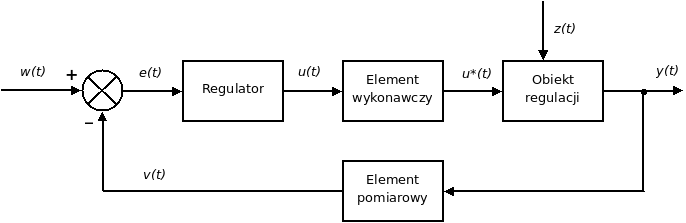
\includegraphics[width=0.5\textwidth]{./graf/regulacja1.png}
    \caption{Rysunek przedstawiający ogólny schemat układu regulacji automatycznej \cite{bib:wiki-regulacja}}
    \label{rys2:regulacja1}
\end{figure}

\subsection{Działanie regulatora PID}

Działanie regulatora PID opiera się na przetwarzaniu sygnału uchybu $e(t)$, czyli różnicy między wartością zadaną $y_{set}$ a wartością rzeczywistą $y(t)$ wielkości regulowanej:

\begin{equation}
e(t) = y_{set} - y(t)
\end{equation}

Regulator PID wyznacza wartość sygnału sterującego $u(t)$ jako sumę trzech składników:
\begin{equation}
u(t) = K_p e(t) + K_i \int_{0}^{t} e(\tau) d\tau + K_d \frac{de(t)}{dt}
\end{equation}
gdzie:
\begin{itemize}
    \item $K_p$ – współczynnik proporcjonalny, który wzmacnia aktualny uchyb,
    \item $K_i$ – współczynnik całkujący, który reaguje na sumę uchybów w czasie,
    \item $K_d$ – współczynnik różniczkujący, który reaguje na zmianę uchybu.
\end{itemize}

Każda ze składowych regulatora PID pełni inną funkcję, a ich kombinacja pozwala na precyzyjne kontrolowanie zachowania systemu.

\subsection{Składnik proporcjonalny $P$}

Składnik proporcjonalny jest liniowo zależny od uchybu $e(t)$ i odpowiada za natychmiastową reakcję na różnicę między wartością zadaną a rzeczywistą. Działa zgodnie ze wzorem:

\begin{equation}
P(t) = K_p e(t)
\end{equation}

Im większa wartość $K_p$, tym regulator bardziej dynamicznie reaguje na uchyb, co może przyspieszyć osiągnięcie wartości zadanej, ale przy zbyt dużych wartościach może prowadzić do przeregulowania lub oscylacji.

\subsection{Składnik całkujący $I$}

Składnik całkujący sumuje uchyby w czasie, co pozwala na eliminację uchybu statycznego – różnicy między wartością rzeczywistą a zadaną, która może utrzymywać się w przypadku stosowania tylko składnika proporcjonalnego. Składnik całkujący jest dany równaniem:

\begin{equation}
I(t) = K_i \int_{0}^{t} e(\tau) d\tau
\end{equation}

Dzięki temu składnikowi, regulator PID potrafi zniwelować długotrwały uchyb, chociaż przy zbyt dużych wartościach $K_i$ może wystąpić zjawisko przeregulowania i niestabilność.

\subsection{Składnik różniczkujący $D$}

Składnik różniczkujący uwzględnia szybkość zmian uchybu $e(t)$, co pozwala na szybsze reagowanie na gwałtowne zmiany i przeciwdziałanie efektowi przeregulowania. Opisuje go wyrażenie:

\begin{equation}
D(t) = K_d \frac{de(t)}{dt}
\end{equation}

Ten składnik regulatora poprawia stabilność i tłumi oscylacje, jednak zbyt duża wartość $K_d$ może prowadzić do niestabilności układu, zwłaszcza w obecności szumów.

\subsection{Pełne równanie regulatora PID}

Łącząc wszystkie trzy składniki, równanie regulatora PID przyjmuje postać:

\begin{equation}
u(t) = K_p e(t) + K_i \int_{0}^{t} e(\tau) d\tau + K_d \frac{de(t)}{dt}
\end{equation}

gdzie:
\begin{itemize}
    \item $K_p e(t)$ – składnik proporcjonalny, który odpowiada za szybką reakcję na zmiany,
    \item $K_i \int_{0}^{t} e(\tau) d\tau$ – składnik całkujący, który eliminuje uchyb statyczny,
    \item $K_d \frac{de(t)}{dt}$ – składnik różniczkujący, który przeciwdziała nagłym zmianom uchybu.
\end{itemize}

Regulacja parametrów $K_p$, $K_i$ i $K_d$ pozwala na dostosowanie charakterystyki regulatora PID do specyfiki sterowanego obiektu. Optymalne wartości tych parametrów zazwyczaj są dobierane metodą prób i błędów lub za pomocą metod takich jak strojenie Zieglera-Nicholsa.

\subsection{Zastosowanie regulatora PID w sterowaniu robotem mobilnym}

W omawianym projekcie regulator PID znajduje zastosowanie w kontrolowaniu odległości jaką pokonuje platforma mobilna poprzez odpowiednie sterowanie napięciem zasilania elementów wykonawczych. Nastawy regulatora zostały dostosowane metodą prób i błędów z racji trdudnego do zamodelowania układu dynamicznego. Uzyskana jakość regulacji jest wystarczająca do spełnienia wymagań projektowych. 

\section{Podstawy wykrywania krawędzi w wizji komputerowej}

Wykrywanie krawędzi stanowi kluczowy element analizy obrazów w kontekście wizji komputerowej. Jest to technika mająca na celu identyfikację istotnych zmian w intensywności pikseli obrazu, które zazwyczaj wskazują na obecność krawędzi obiektów. Krawędzie odgrywają fundamentalną rolę w percepcji kształtów i struktur, dlatego ich wykrywanie jest podstawą wielu aplikacji, takich jak segmentacja obrazu, rozpoznawanie obiektów oraz analiza ruchu.

Jedną z najbardziej popularnych metod wykrywania krawędzi jest algorytm Canny’ego, który został zaproponowany przez Johna F. Canny'ego w 1986 roku. Metoda ta jest ceniona za swoją zdolność do wydobywania krawędzi z obrazów przy jednoczesnym zachowaniu ich jakości oraz redukcji szumów.

\subsection{Algorytm Canny’ego}

Algorytm Canny’ego składa się z kilku kluczowych kroków:

1. \textbf{Wygładzenie} (ang. \english{Smoothing}): Na początku obraz poddawany jest filtracji w celu zredukowania szumów. Zazwyczaj stosuje się filtr Gaussa, który jest reprezentowany przez macierz:

\[
G = \begin{bmatrix}
\frac{1}{16} & \frac{1}{8} & \frac{1}{16} \\
\frac{1}{8} & \frac{1}{4} & \frac{1}{8} \\
\frac{1}{16} & \frac{1}{8} & \frac{1}{16}
\end{bmatrix}
\]

2. \textbf{Obliczenie gradientu:} Następnie obliczane są gradienty obrazu, aby zidentyfikować kierunki zmian intensywności. Używa się do tego macierzy \textit{Sobela}, które pozwalają na obliczenie gradientu w kierunkach poziomym (Gx) i pionowym (Gy):

\[
S_x = \begin{bmatrix}
-1 & 0 & 1 \\
-2 & 0 & 2 \\
-1 & 0 & 1
\end{bmatrix}, \quad 
S_y = \begin{bmatrix}
1 & 2 & 1 \\
0 & 0 & 0 \\
-1 & -2 & -1
\end{bmatrix}
\]

Gradient można obliczyć jako:

\[
G = \sqrt{G_x^2 + G_y^2}
\]
oraz jego kierunek:

\[
\Theta = \text{atan2}(G_y, G_x)
\]

3. \textbf{Tłumienie nie-maksymalne} (ang. \english{Non-maximum suppression}): W kolejnym kroku następuje eliminacja pikseli, które nie są lokalnymi maksimami w kierunku gradientu, co pozwala na wyostrzenie krawędzi.

4. \textbf{Podwójne progowanie} (ang. \english{Double thresholding}): Algorytm wprowadza dwa progi: wysoki i niski. Piksele, które przekraczają wysoki próg, są uznawane za krawędzie, natomiast te, które są poniżej niskiego progu, są odrzucane. Piksele, które mieszczą się między tymi dwoma progami, są klasyfikowane jako krawędzie słabe.

5. \textbf{Śledenie krawędzi z histerezą} (ang. \english{Edge tracking by hysteresis}): Ostatnim krokiem jest śledzenie krawędzi, gdzie słabe krawędzie są zachowywane, jeśli są połączone z mocnymi krawędziami. To pozwala na eliminację przypadkowych detekcji krawędzi i zapewnia spójność wyników.

\clearpage

\section{Podstawy rozpoznawania kolorów w wizji komputerowej}

Rozpoznawanie kolorów w wizji komputerowej to kluczowy aspekt w wielu aplikacjach automatyki, robotyki oraz sztucznej inteligencji. W kontekście robotyki, techniki te pozwalają na identyfikację i klasyfikację obiektów w otoczeniu robota, co jest istotne dla jego nawigacji oraz interakcji z otoczeniem. W niniejszej sekcji omówione zostaną podstawowe zasady oraz techniki wykorzystywane w procesie rozpoznawania kolorów.

\subsection{Teoria koloru}


Kolor jest percepcją widzialnego spektrum światła, które jest odbierane przez ludzkie oczy i interpretowane przez mózg. W wizji komputerowej kolory są często reprezentowane za pomocą różnych modeli kolorów, w tym w przestrzeni kolorów RGB (ang. \english{Red, Green, Blue}) \textit{rys.} [\ref{rys2:rgb1}], HSV (ang. \english{Hue, Saturation, Value}) \textit{rys.} [\ref{rys2:hsv1}] oraz YCrCb (ang. \english{Luminance, Chrominance}) \textit{rys.} [\ref{rys2:ycrcb1}]. W modelu RGB kolory są definiowane przez intensywności trzech składowych kolorów, podczas gdy w modelu HSV kolory są określane na podstawie ich odcienia, nasycenia i jasności, co ułatwia przetwarzanie i rozpoznawanie kolorów w kontekście wizji komputerowej. Model YCrCb, z kolei, oddziela informację o luminancji (jasności) od informacji o chrominancji (kolorze), co jest szczególnie przydatne w kompresji obrazów oraz w systemach wizyjnych, umożliwiając efektywną analizę kolorów przy jednoczesnym zredukowaniu wpływu zmian oświetleniowych.


\begin{figure}[H]
    \centering
    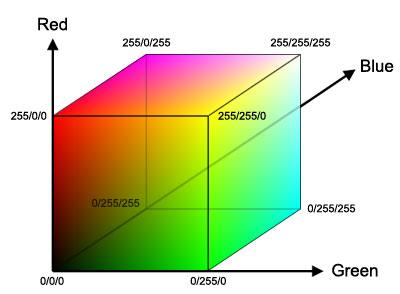
\includegraphics[width=0.6\textwidth]{./graf/rgb-model.png}
    \caption{Rysunek przedstawiający wizualizację przestrzeni kolorów RGB \cite{bib:rgb-model}}
    \label{rys2:rgb1}
\end{figure}

\begin{figure}[h]
    \centering
    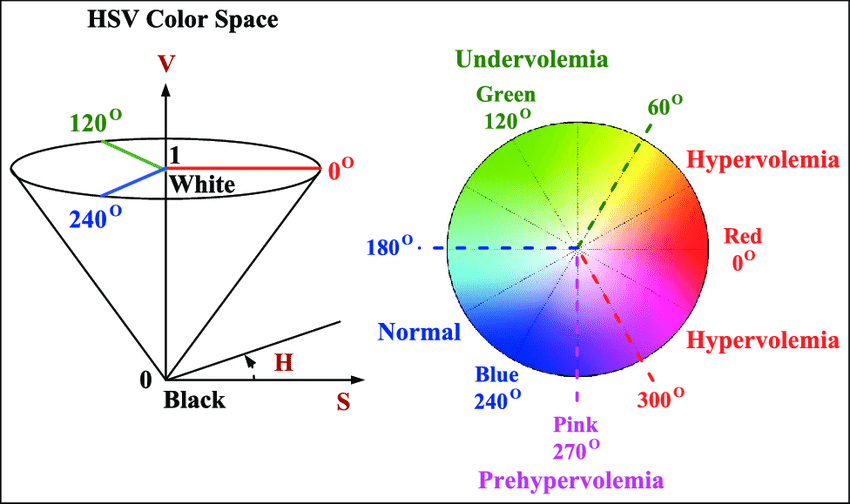
\includegraphics[width=0.6\textwidth]{./graf/hsv-model.png}
    \caption{Rysunek przedstawiający wizualizację przestrzeni HSV \cite{bib:hsv-model}}
    \label{rys2:hsv1}
\end{figure}


\begin{figure}[h]
    \centering
    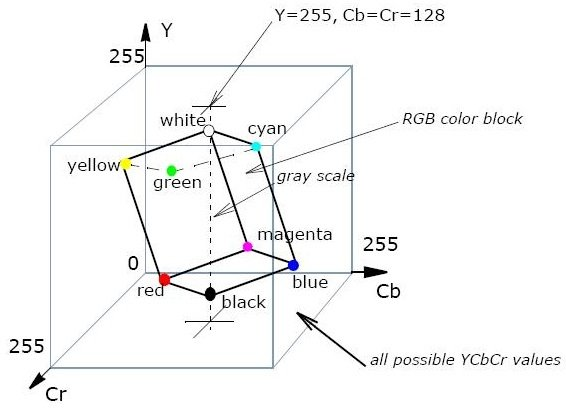
\includegraphics[width=0.6\textwidth]{./graf/ycrcb-model.png}
    \caption{Rysunek przedstawiający wizualizację przestrzeni YCrCb \cite{bib:ycrcb-model}}
    \label{rys2:ycrcb1}
\end{figure}

\clearpage

\subsection{Proces rozpoznawania kolorów}

Proces rozpoznawania kolorów w obrazach polega na identyfikacji oraz klasyfikacji pikseli na podstawie ich wartości kolorystycznych. Kluczowe etapy tego procesu obejmują:

\begin{enumerate}
    \item \textbf{Przechwytywanie obrazu:} Obraz jest przechwytywany za pomocą kamery cyfrowej, która generuje dane w formacie cyfrowym. 
    \item \textbf{Przetwarzanie obrazu:} Na tym etapie obraz jest poddawany różnym operacjom, takim jak filtracja, segmentacja i transformacja kolorów, aby wyodrębnić istotne informacje. 
    \item \textbf{Ekstrakcja cech:} Następnie przeprowadzana jest analiza danych kolorystycznych w celu identyfikacji i klasyfikacji obiektów na podstawie ich kolorów. 
    \item \textbf{Decyzja:} Na końcu system podejmuje decyzje o klasifikacji obiektów bazując na wcześniej zebranych informacjach o kolorze.
\end{enumerate}

\subsection{Algorytmy rozpoznawania kolorów}

W literaturze przedmiotu opisano wiele algorytmów wykorzystywanych w rozpoznawaniu kolorów, w tym metody oparte na histogramie, segmentacji obrazu oraz analizy cech. Histogramy kolorów są popularnym narzędziem do analizy rozkładu kolorów w obrazie, co pozwala na szybką identyfikację dominujących kolorów.

Segmentacja obrazu to proces dzielenia obrazu na różne regiony na podstawie ich kolorów, co ułatwia identyfikację obiektów w danym kolorze. Algorytmy takie jak k-means clustering czy metoda watershed są często stosowane w celu wydzielenia obiektów o określonym kolorze z tła.

DO POPRAWY - TRZEBA DO JESZCZE SENSOWNIE OPISAĆ (!!!!)